\FILE{interfaces.tex}

\section{Cloudmesh-cc Interfaces}

In this section we explain the various ways of interfacing with
cloudmesh-cc that are part of our design (see Figure~\ref{fig:arch}).

It is important to note that we have a {\em commandline mode} that interfaces directly with the backends while not requiring a service. This includes an easy-to-use Python API.

In addition, we have used this API to implement a {\em service mode}, so we can stand up a REST service as well as a GUI that can be accessed through a Web browser.
Please note that the service mode can also be accessed through the command line in a terminal. To distinguish how we operate cloudmesh-cc we use the term {\em mode} to delineate it from a command that is entered in a terminal to query the status of the workflow.

We will now discuss these interfaces in more detail and also showcase
how we can access them.


\subsection{Python API}

Cloudmesh-cc is implemented in Python. Extensive documentation is
available in GitHub and through GitHub action it is automatically
updated \cite{github-cloudmesh-cc}.  We distingush two main classes
that are easy to use. The first is a {\em Job class} that can be adapted
to include new computational resource types for executing jobs. The
second is a {\em Workflow class} to coordinate the execution of
multiple jobs. Selected methods of the Job class include are listed in
Figure~\ref{fig:code-job}. Important to note is that the code for the
scripts are all managed locally and a synchronization step is invoked
prior to one running the job to assure that the latest script and
code to be executed on the compute resource is available.

The most important part of using the Workflow Python API is showcased
in Figure~\ref{fig:code-job}, where we explain how easy it is to set up a workflow
with the Python API.

\begin{figure}[!h]
\begin{minted}[breaklines]{bash}
class Job:
   ...
   def clear():
      """Clear job progress."""
   def create(filename=None, script=None, exec=None):
      """Create a template for the script with progress."""
   def get_log(refresh=True):
      """Get the log of the job."""
   def get_pid(refresh=False):
      """Get the pid that the job is running within determined by the compute resource it is running on."""
   def get_progress(refresh=False):
       """Get the progress of the job from the compute resource."""
   def get_status(refresh=False):
       """Get the status of the job."""
   def kill():
       """Kill the job."""
   def run():
       """Run the job."""
   def sync():
       """Synchronise the current directory with the remote. Copies the shell script to the experiment directory and ensures that the file is copied with the sync command."""
   def watch(period=10):
       """Watch the job and check for changes in the given period."""
\end{minted}
\caption{Pseudo code for the Job class with selected methods.}
\label{fig:code-job}

\bigskip

\begin{minted}[breaklines]{bash}
class Workflow:
    ...
    def add_dependencies(dependency):
        """Add a job dependency to the workflow (and the graph)."""
    def add_dependency(source, destination):
        """Add a job dependency to the workflow (and the graph)."""
    def add_job( ... ):
        """Add a job to the workflow with appropriate parameters."""
    def display(filename=None, name='workflow', first=True):
        """Show the graph of the workflow."""
    def job(name):
        """Return the details of a job within the workflow."""
    def load(filename, clear=True):
        """Load the workflow."""
    def remove_job(name, state=False):
        """Remove a particular job from the workflow."""
    def remove_workflow():
        """Delete workflow from the local file system."""
    def run_parallel( ... ):
        """Run a workflow in a parallel fashion."""
    def run_topo(order=None, dryrun=False, show=True, filename=None):
        """Run the workflow in a topological order."""
    def save(filename=None):
        """Save the workflow."""
    def save_with_state(filename, stdout=False):
        """Save the workflow with state."""
    def sequential_order():
        """Return a list of the topological order of the workflow."""
    property table:
        """Return a table of the workflow."""
    def update_progress(name):
        """Manually update the progress of a job according to its log file."""
    def update_status(name, status):
        """Manually update a job’s status."""
\end{minted}
\caption{Pseudo code for the Job class with selected methods.}
\label{fig:code-workflow}
\end{figure}


\begin{figure}[htb]
\begin{minted}[breaklines]{bash}
    w = Workflow(name="workflow-analyze")
    # load a preexisting workflow
    # w.load(filename="source.yaml")
    
    # add jobs and dependencies explicitly
    w.add_job(name="fetch-data",
              exec="hostname",
              host="supercomputer-a", # defined in .ssh
              label="{name}\nprogress={progress}",
              kind="local",
              status="ready",
              progress=0)
    w.add_job(name="compute", command="... TBD ...")
    w.add_job(name="analyze", command="... TBD ...")
    w.add_dependencies(
              dependency="start,fetch-data,compute,analyze")
    w.run_topo()
\end{minted}
\caption{Pseudo code for the Job class with selected methods.}
\label{fig:code-workflow-example}

\bigskip

\begin{minted}[breaklines]{bash}
      cms cc workflow add [--name=NAME] [--job=JOB] ARGS...
      cms cc workflow add [--name=NAME] --filename=FILENAME
      cms cc workflow delete [--name=NAME] [--job=JOB]
      cms cc workflow list [--name=NAME] [--job=JOB]
      cms cc workflow run [--name=NAME] [--job=JOB] [--filename=FILENAME]
      cms cc workflow [--name=NAME] --dependencies=DEPENDENCIES
      cms cc workflow status --name=NAME [--output=OUTPUT]
      cms cc workflow graph --name=NAME
\end{minted}
\caption{Command line interface to the workflow in terminal mode.}
\label{fig:code-workflow-commandline}

\bigskip

\begin{minted}[breaklines]{bash}
      cms cc start [-c] [--reload] [--host=HOST] [--port=PORT]
      cms cc stop
      cms cc status
      cms cc workflow service add [--name=NAME] FILENAME
      cms cc workflow service list [--name=NAME] [--job=JOB]
      cms cc workflow service add [--name=NAME] [--job=JOB] ARGS...
      cms cc workflow service run --name=NAME
\end{minted}
\caption{Command line interface to the workflow in service mode.}
\label{fig:code-workflow-service-commandline}.

% \bigskip

{\centering
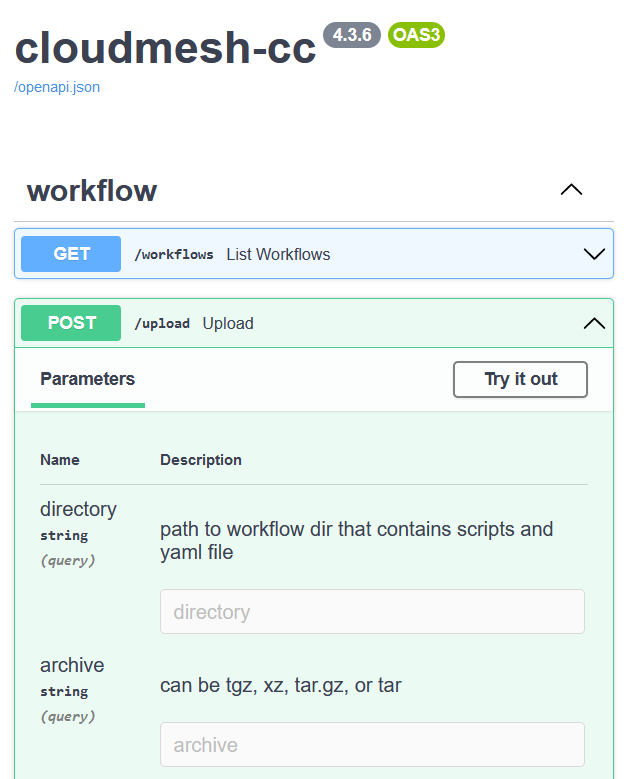
\includegraphics[width=0.52\columnwidth]{images/upload_api.png}
}
\caption{Browser API GUI for Cloudmesh Compute Cluster.}

\label{fig:openapi}

\end{figure}


\subsection{Commandline Mode}

The commandline mode is an implementation that does not use a backend
service. It runs in the terminal until the workflow is completed. All
states of the jobs are managed on the compute service on which the job
is run and the status is replicated into the client on demand. This
allows easy reporting of the status through a table and a graph
display using client based rendering tools. The various commands to
interact with it on the commandline are shown in
Figure~\ref{fig:code-workflow-commandline}.


\subsection{Service Mode}

The Python API has been used to implement a REST service. To
easily interact with the REST service we have also added a couple of
convenient commands one can issue from a terminal. They are listed
in Figure~\ref{fig:code-workflow-service-commandline}. It is clear for
these methods that starting, stopping, and getting the status of the
service is very easy. In contrast to the commandline mode this service
mode has an additional keyword {\em service} to interact with the rest service.

Certainly one can also directly interact with the REST service API for
this service. For ease of use, we have exposed the interface through
an OpenAPI specification that is available to the user as shown in
Figure~\ref{fig:openapi}.

Thus, other tools such as curl or other languages supporting url
requests can be used. A curl example to list the workflow
specifications uploaded to the service is as follows:

\begin{minted}[breaklines]{bash}
$ curl -X 'GET' \
    'http://127.0.0.1:8000/workflows' \
    -H 'accept: application/json'
\end{minted}

As we use a REST service, we can also easily upload the workflow
through a Python enabled REST call. We will use Python requests to
demonstrate this upload feature. To showcase the various ways to
access the service we focus on uploading a tar file that contains the
workflow as well as the scripts or programs used in the workflow. The
tar file is called {\em workflow.tar}.

To also allow programming against the REST service in Python, a Python
API similar to that of the commandline mode is
available. Figure~\ref{fig:code-workflow-rest-commandline} showcases
this API.

To simplify interaction with the REST service we create a special
RESTWorkflow class that is similar to the command module API but uses
instead the REST interface to the service rather than direct
communication with the command client API.

The user can also simply use the requests module in Python to
interface with the API. Figure~\ref{fig:code-workflow-requests}
demonstrates how to use requests to upload a workflow by using
an archive file that contains the YAML configuration file and the scripts.

\begin{figure}[t]
\begin{minted}[breaklines]{bash}
class RESTWorkflow
    ...
    def add_job(workflow_name, **kwargs):
        """Add a job to the workflow."""
    def delete_workflow(workflow_name, job_name=None):
        """Delete a workflow by using REST."""
    def get_workflow(workflow_name, job_name=None):
        """Retrieve a workflow by using REST."""
    def list_workflows():
        """Return a list of workflows that is found within
           the server."""
    def run_workflow( ... ):
        """Run a workflow by using REST."""
    def upload_workflow( ... ):
        """Upload a workflow by using REST."""
\end{minted}
\caption{Pseudo code for the Job class with selected methods.}
\label{fig:code-workflow-rest-commandline}

\bigskip

\begin{minted}[breaklines]{python}
import requests
r = requests.post(
      'http://127.0.0.1:8000/workflow?archive=workflow-example.tar')
print(r.text)
\end{minted}
\caption{Upload to the REST service with Python requests.}
\label{fig:code-workflow-requests}

\bigskip

\begin{minted}[breaklines]{bash}
$ curl -X 'POST' 'http://127.0.0.1:8000/ workflow?archive=workflow-example.tar'                           -H 'accept: application/json' -d ''
\end{minted}%$
\caption{Upload to the REST service with curl.}
\label{fig:code-workflow-curl}

\end{figure}


\subsection{Webservice GUI}

A convenient Web service is included in Cloudmesh cc. It allows the user
to manage and visualize the status of workflows through a Web browser
interface. At this time the focus is that the interface can be run by a
singleuser on the local machine. This allows that remote executions of
workflow nodes run completely independent from cloudmesh cc and
interaction is possible in asynchronous mode.

As the service is using also an OpenAPI 2.0 specification the workflow
can also be uploaded implicitly through the specification

GUI. Navigate to {\scriptsize \texttt{http://127.0.0.1:8000/docs}} and
use the POST Upload method. Then click \texttt{Try\ it\ out} and enter
the

location of the tar file, followed by clicking {\em Execute}.

Obviously, any REST service or REST API can be used allowing to
interface to it from different programming languages or frameworks.

The web server provides a more customizable, easy-to-use interface for
the Workflow class which can be started, viewed, and stopped with the
appropriate command line. 

\begin{minted}[breaklines]{bash}
  $ cms cc start
  $ cms cc view
  $ cms cc stop
\end{minted}%$


The view can also be achieved by opening the 
the link {\scriptsize\texttt http://127.0.0.1:8000/}.

Now the browser provides an interface to view preexisting workflows in both
a DataTable format and as a graph format. Both views will update
automatically, in a live fashion, as the workflows are run, reporting
live job status and progress.

For a quick and easy example of leveraging this GUI interface, click
n the Example tab in the left-hand sidebar. Then, a workflow-example
will appear underneath Workflows. Click on the workflow-example and
run the workflow by clicking the green Run button in the top-right. As
the workflow runs, the user is able to click on the Graph button
to view the graph interface (see Figure~\ref{fig:graph}) and back to the
Table button for the table interface (see Figure~\ref{fig:table}), as
desired, to view the workflow's progression.


\begin{figure}[htb]
{\centering
  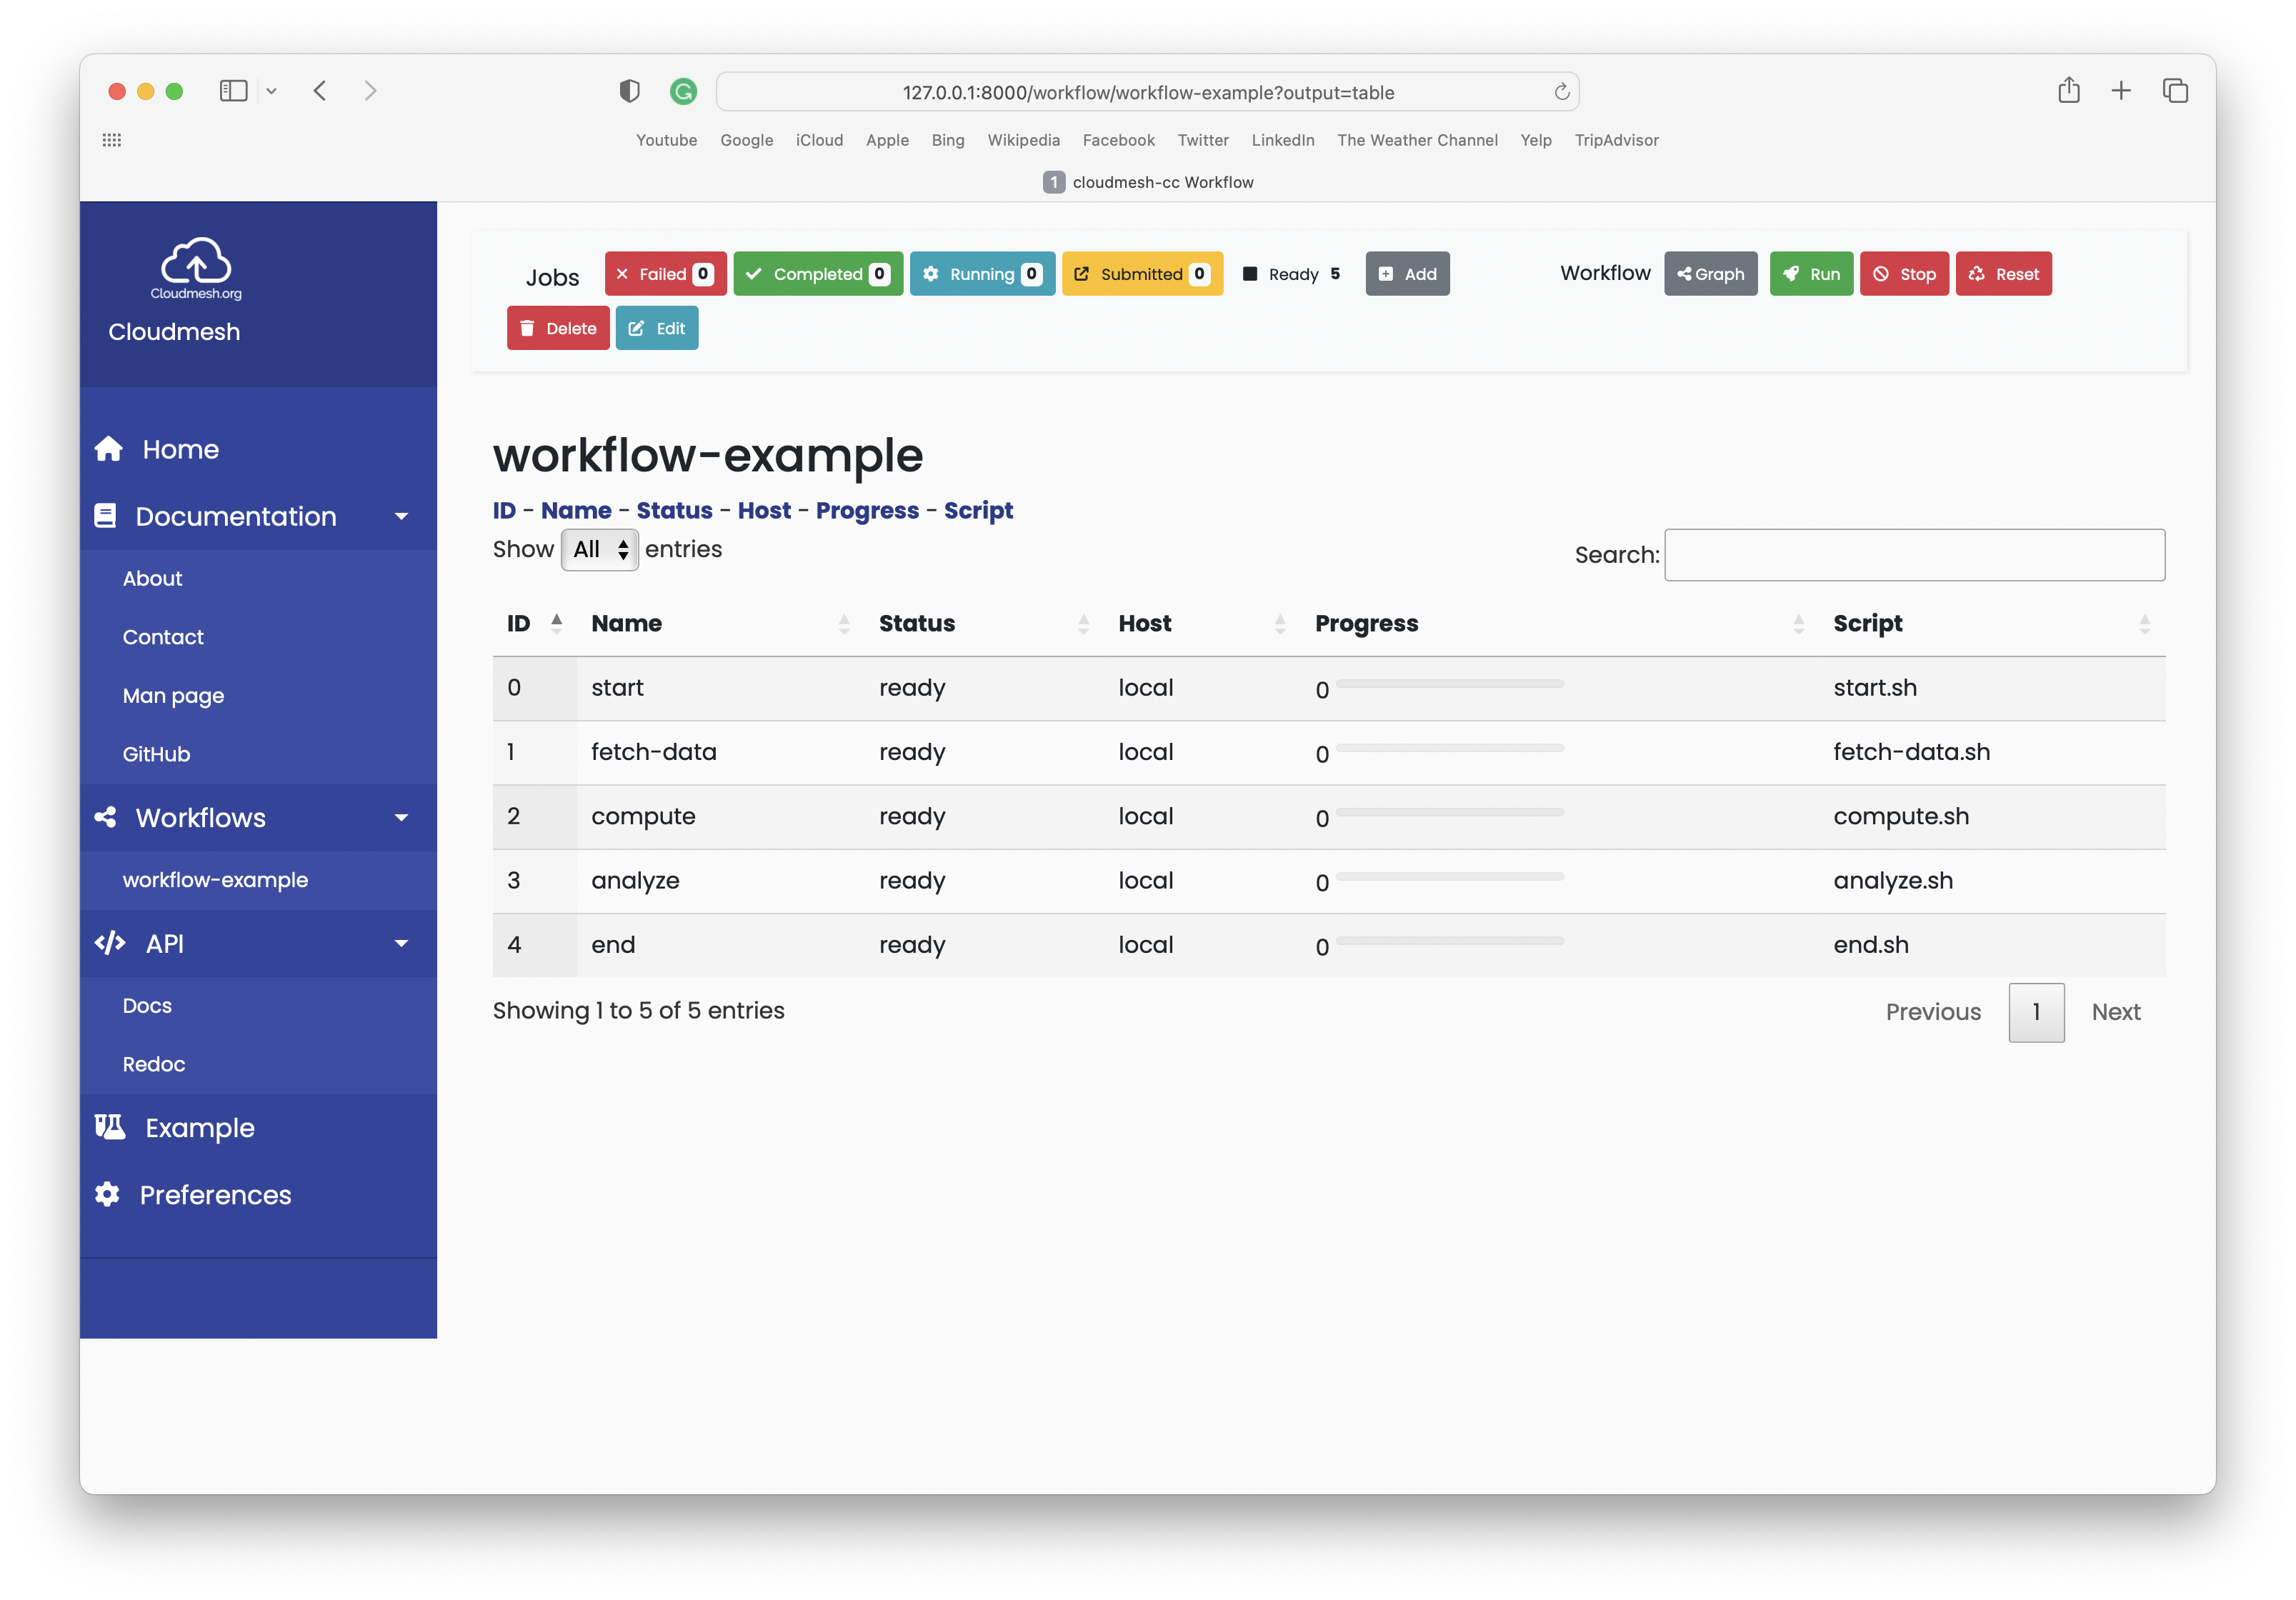
\includegraphics[width=1.0\columnwidth]{images/service-table.png}
}
\vspace{-1.0cm}
\caption{Cloudmesh cc workflow table view.}\label{fig:table}

\bigskip
{\centering
  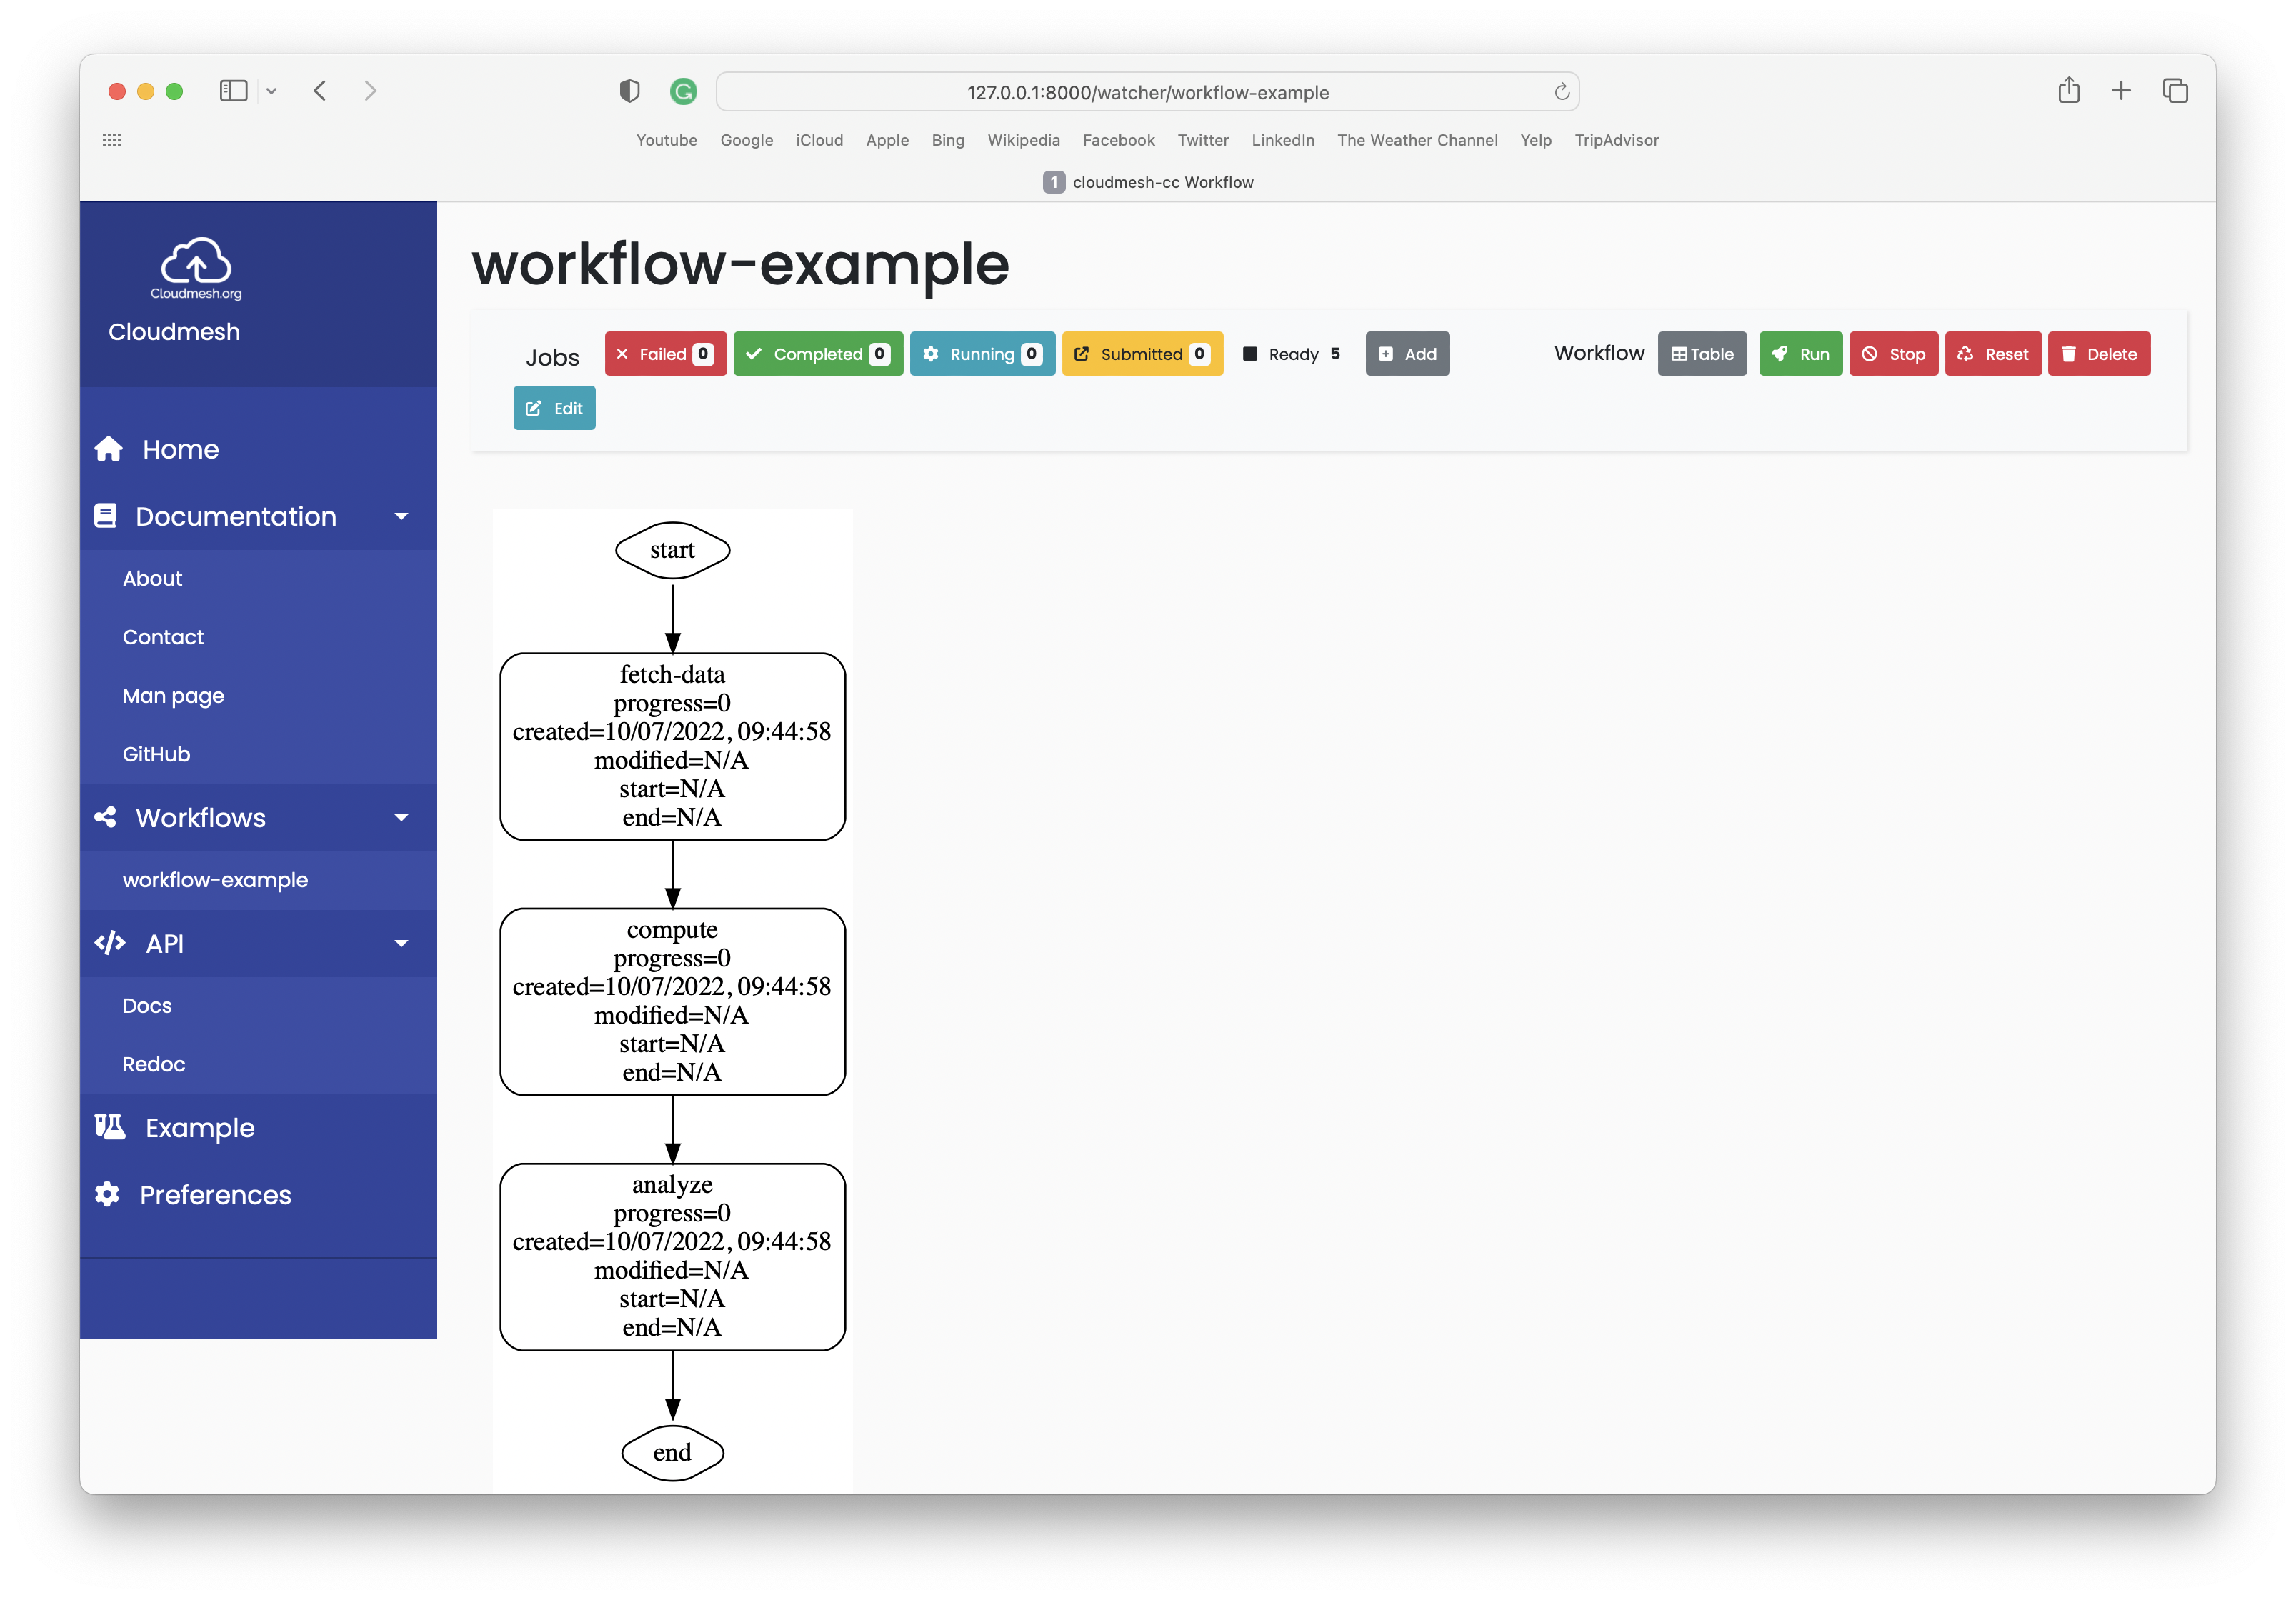
\includegraphics[width=1.0\columnwidth]{images/service-graph.png}
 }
\vspace{-1.0cm}
 \caption{Cloudmesh cc workflow graph view.}

\label{fig:graph}
\end{figure}



\subsection{Run the workflow}\label{run-the-workflow}

The workflow can be run easily via the GUI. We added a special set of
buttons to the workflow table and graph display to simplify running of
the workflow. 
Nevertherless, certainly the workflow can also be activated while
calling the appropriate REST call, either through, Python, the OpenAPI
docs page, or, for example, a curl call such as
where {\em workflow-example} is the name of the workflow to be
executed. Figure~\ref{fig:workflow-run-a}-{fig:workflow-run-c} showcases various methods to
run the example workflow.


\begin{figure}[htb]

\begin{minted}[breaklines]{bash}
$ curl -X 'GET' 'http://127.0.0.1:8000/workflow/run/workflow-example?show=True' -H 'accept: application/json'
\end{minted}%$
\flushleft
\caption{\parindent0pt Running the example workflow with curl.}
\label{fig:workflow-run-a}
\bigskip

\begin{minted}[breaklines]{python} 
from cloudmesh.cc.workflowrest import RESTWorkflow
rest = RESTWorkflow()
result = rest.run_workflow('workflow-example')
\end{minted}

\caption{Running the example workflow with cloudmesh RESTWorkflow API.}
\label{fig:workflow-run-b}
\bigskip

\begin{minted}[breaklines]{python}
import requests
url = f'http://127.0.0.1:8000/workflow/run/workflow-example?show=True'
r = requests.get(url)
print(r)
\end{minted}

\caption{Running the example workflow with requests API.}
{fig:workflow-run-c}

\end{figure}




